\chapter{Magnetic Fields}

We start the study of two-dimensional quantum dots under the influence of a magnetic 
field by defining a system of only one particle and solving the time-dependent 
Schrödinger equation
directly. This is a accomplished by using the \lstinline{TwoDimHarmonicOscB} class
to produce a basis set, single-particle functions and transition/intearction matrix (dipole elements),
which is everything we need. All of these items are properties of the class and can be
easily extracted. A simple periodic function simulates an electric field is constructed, as 
the product of such a time-dependent operator and the interaction matrix defines the 
time propagation. We then use a simple integration scheme, in this case the fourth-order 
Runge-Kutta method, to propagate the ground state single particle function of the system.
Taking care to extract the dipole for every time step, we can compute the discrete Fourier 
transform of the dipole and compute the frequency spectrum of our system. This procedure is 
applied to a system comletely absent of a magnetic field, and a system under direct influence 
of a magnetic field.

Before going straight to the results, we study the shell structure and allowed transitions of 
our two systems. The left part of \autoref{fig:shell_structure_yes_no_b} presents the 
shell structure of a the regular two-dimensional quantum dot. The states have all been assigned
a number for easier examination. This shell structure is 
identical to the one presented in \autoref{fig:2d_basis_states}. Additionally, here we have added
coloured double arrows to illustrate the allowed transitions in the quantum dot. These 
transitions are can be encountered in the transition matrix for the system, which is
reproduced in the artistic way in \autoref{fig:transition_no_b}. Notice that the coloured 
arrows representing allowed transitions match in colour with the elements of the transition 
matrix.

\begin{figure}
    \begin{center}
    \begin{tikzpicture}[scale=0.9, background rectangle/.style={fill=grey},
        show background rectangle]
    \begin{scope}
      
        % TOP
        \foreach \i in {0, 3, 6} {
            \draw(\i, 2) -- (\i + 2, 2);
            \node at (\i + 0.75, 2) {$\uparrow$};
            \node at (\i + 1.25, 2) {$\downarrow$};
        }
       
        \node[below, inner sep=.5em] at (1, 2) {$(0, -2)$};
        \node[above] at (1, 2) {5};
        \node[below, inner sep=.5em] at (4, 2) {$(1, 0)$};
        \node[above] at (4, 2) {3};
        \node[below, inner sep=.5em] at (7, 2) {$(0, 2)$};
        \node[above] at (7, 2) {4};

        % MIDDLE
        \foreach \i in {1.5, 4.5} {
            \draw(\i, 1) -- (\i + 2, 1);
            \node at (\i + 0.75, 1) {$\uparrow$};
            \node at (\i + 1.25, 1) {$\downarrow$};
        }

        \node[below, inner sep=.5em] at (2.5, 1) {$(0, -1)$};
        \node[above] at (2.5, 1) {1};
        \node[below, inner sep=.5em] at (5.5, 1) {$(0, 1)$};
        \node[above] at (5.5, 1) {2};

        % BOTTOM
        \draw(3, 0) -- (5, 0);
        \node at (3 + 0.75, 0) {$\uparrow$};
        \node at (3 + 1.25, 0) {$\downarrow$};

        \node[below, inner sep=.5em] at (4, 0) {$(0, 0)$};
        \node[above] at (4, 0) {0};

        % Transitions
        \draw [<->, line width=.1em, transition11] (3.5, 0) -- (3.25, 1);
        \draw [<->, line width=.1em, transition11] (4.5, 0) -- (4.75, 1);

        \draw [<->, line width=.1em, transition12] (3, 1) -- (3.25, 2);
        \draw [<->, line width=.1em, transition12] (5, 1) -- (4.75, 2);

        \draw [<->, line width=.1em, transition13] (2, 1) -- (1.75, 2);
        \draw [<->, line width=.1em, transition13] (6, 1) -- (6.25, 2);

    \end{scope}

    \begin{scope}[xshift=20em]

        % MIDDLE 2
        \foreach \i in {1.5, 4.5} {
            \draw(\i, 3) -- (\i + 2, 3);
            \node at (\i + 0.75, 3) {$\uparrow$};
            \node at (\i + 1.25, 3) {$\downarrow$};
        }

        \node[below, inner sep=.5em] at (2.5, 3) {$(1, 0)$};
        \node[above] at (2.5, 3) {3};
        \node[below, inner sep=.5em] at (5.5, 3) {$(0, 3)$};
        \node[above] at (5.5, 3) {6};

        % MIDDLE 1
        \foreach \i in {1.5, 4.5} {
            \draw(\i, 2) -- (\i + 2, 2);
            \node at (\i + 0.75, 2) {$\uparrow$};
            \node at (\i + 1.25, 2) {$\downarrow$};
        }

        \node[below, inner sep=.5em] at (2.5, 2) {$(0, -1)$};
        \node[above] at (2.5, 2) {1};
        \node[below, inner sep=.5em] at (5.5, 2) {$(0, 2)$};
        \node[above] at (5.5, 2) {4};

        % BOTTOM 2
        \draw(3, 1) -- (5, 1);
        \node at (3 + 0.75, 1) {$\uparrow$};
        \node at (3 + 1.25, 1) {$\downarrow$};

        \node[below, inner sep=.5em] at (4, 1) {$(0, 1)$};
        \node[above] at (4, 1) {2};
        
        % BOTTOM 1
        \draw(3, 0) -- (5, 0);
        \node at (3 + 0.75, 0) {$\uparrow$};
        \node at (3 + 1.25, 0) {$\downarrow$};

        \node[below, inner sep=.5em] at (4, 0) {$(0, 0)$};
        \node[above] at (4, 0) {0};
        
        % Transitions 

        % 0 -> 1
        \draw [<->, line width=.1em, transition21] (3.5, 0) to[out=120, in=-90] (1.75, 2);
        % 0 -> 2
        \draw [<->, line width=.1em, transition21] (4.5, 0) -- (4.5, 1);

        % 2 -> 3
        \draw [<->, line width=.1em, transition23] (3.5, 1) to[out=60, in=-50] (3.25, 3);
        % 2 -> 4
        \draw [<->, line width=.1em, transition22] (4.75, 1) -- (4.75, 2);

        % 1 -> 3
        \draw [<->, line width=.1em, transition23] (2, 2) -- (2, 3);
        % 4 -> 6 
        \draw [<->, line width=.1em, transition24] (6, 2) -- (6, 3);

    \end{scope}
    \end{tikzpicture}
    \end{center} 
    \caption{Shell structure of six lowest orbitals before (left), and after (right)
        a magnetic field is applied to a 2D quantum dot.}
    \label{fig:shell_structure_yes_no_b}
\end{figure}

When we apply apply a magnetic field of strength $\omega_c/\omega = \sqrt{2}/2$ we 
obtain the shell structure represented to the right in 
\autoref{fig:shell_structure_yes_no_b}, where the allowed transitions correpsond to the 
transition matrix in \autoref{fig:transition_yes_b}. The chosen magnetic field strength 
was not chosen arbitrarily, as these accidental degenracies occur only rarely as 
a function of magnetic field strength\footnote{Hence the term ``accidental''.}.
For succinctness we repeat the function for energy eigenvalues for two-dimensional 
quantum dot influenced by a magnetic field (\autoref{eq:2d_b_eigenvalues}),
\begin{equation}
    \epsilon_{nm} = \hbar\Omega(2n + |m| + 1) - \frac{\hbar\omega_c}{2}m,
\end{equation}
where $\Omega = \sqrt{\omega_0^2 + \frac{\omega_c^2}{4}}$.
Apart from a general shift up in energy by adding a magnetic field, the states with 
negative azimuthal quantum number $m$ will experience an increase in energy eigenvalue,
and vice versa. We see this effect clearly in the new shell structure in
\autoref{fig:shell_structure_yes_no_b}. The states with negative $m$ have indeed
undergone a relative shift upwards, whilst the states with positive $m$ have been
shifted downwards, relative to the other states. The ground state, labelled 0, 
remains relatively stationary, the states labelled 2 ($m=1$) and 4 ($m=2$) have been 
shifted downwards and the states labelled 1 ($m=-1$) and 5 ($m=-2$) have been shifted 
upwards. State number 5 so much that it has disappeared from the shell structure, with a 
new state 6 ($=3$) appearing. This is due to our restriction to include only the six
lowest-energy orbitals. We see that the possible remaining allowed transitions remain the 
same, with the exception of transitioning between state 1 and 5, because state 5 is no more,
and the addition of a possible transition between state 4 and 6.

\begin{figure}
    \begin{center}
    \begin{minipage}{0.49\textwidth}
        \centering
        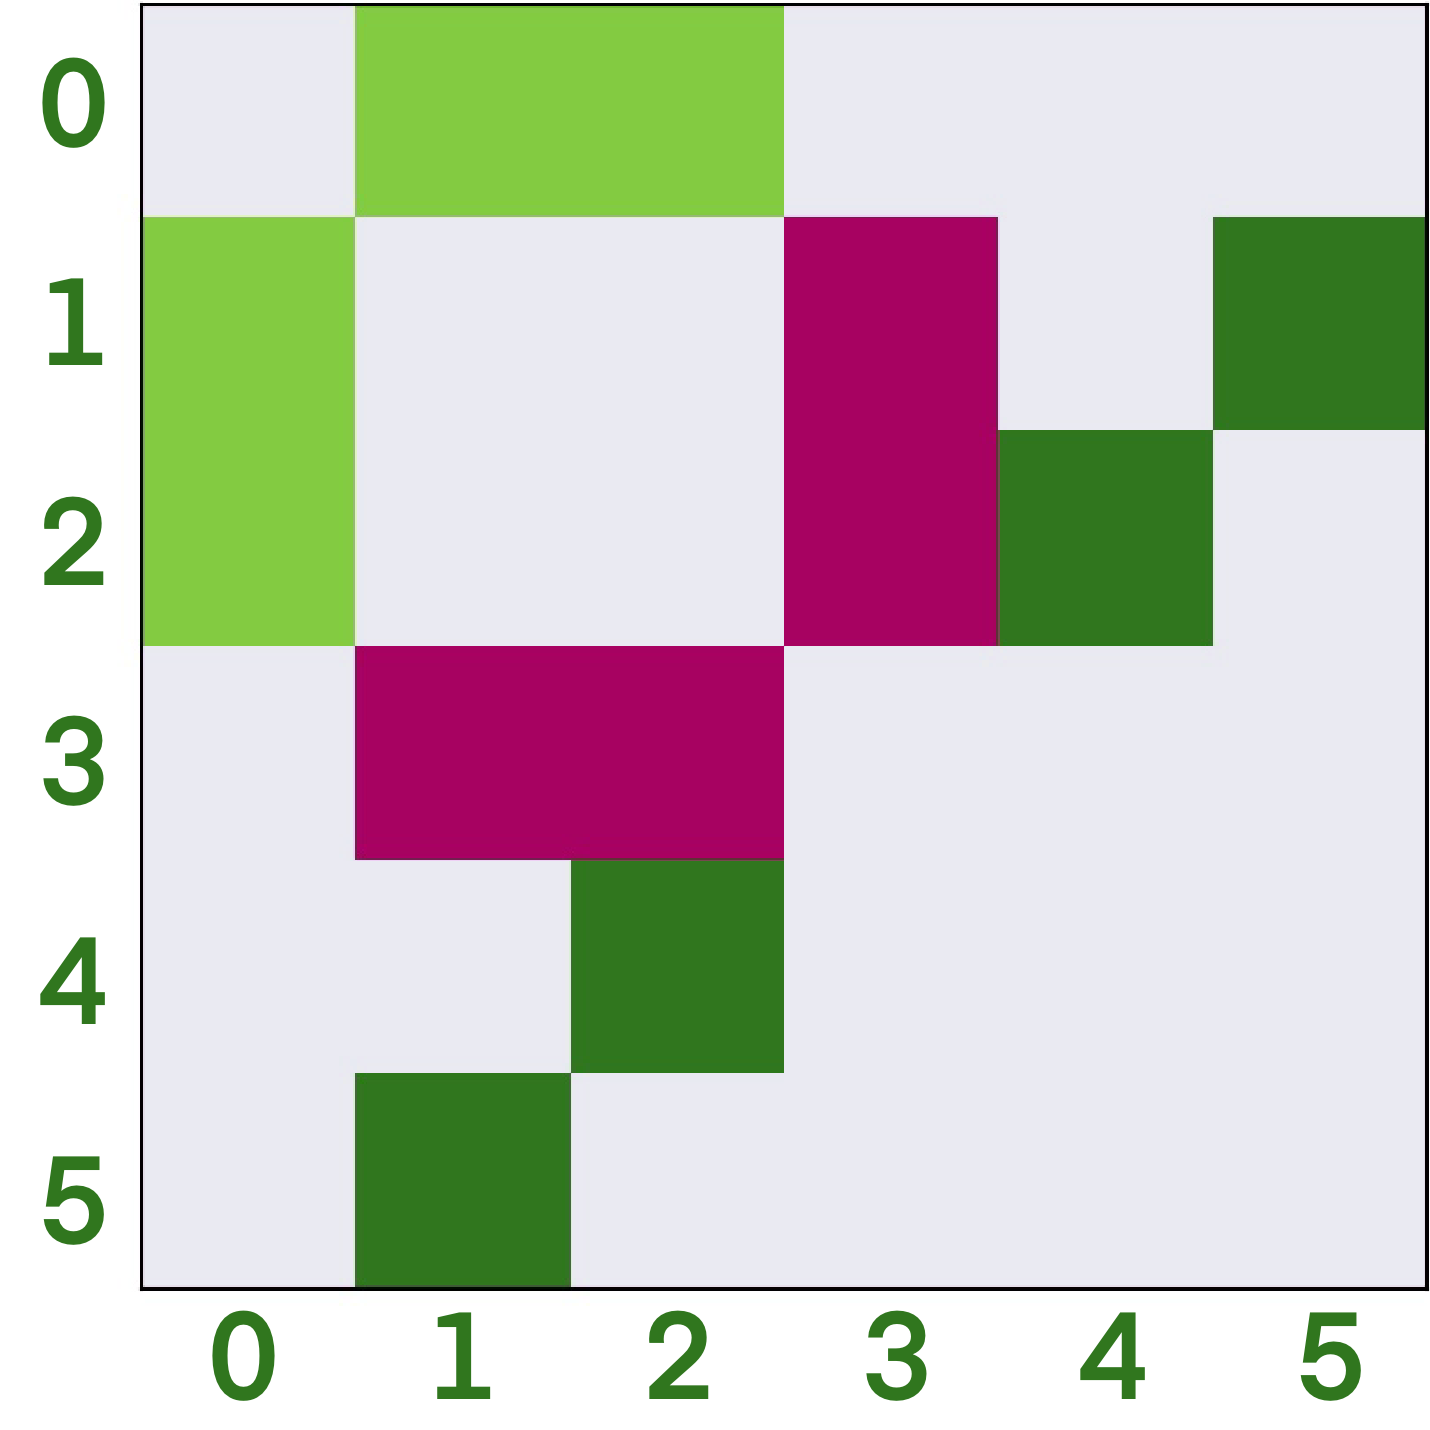
\includegraphics[width=\textwidth]{results/figures/dipole_no_b.png}
        \caption{Transition matrix dictating the allowed transitions for a
            2D quantum dot.}
        \label{fig:transition_no_b}
    \end{minipage}
    \begin{minipage}{0.49\textwidth}
        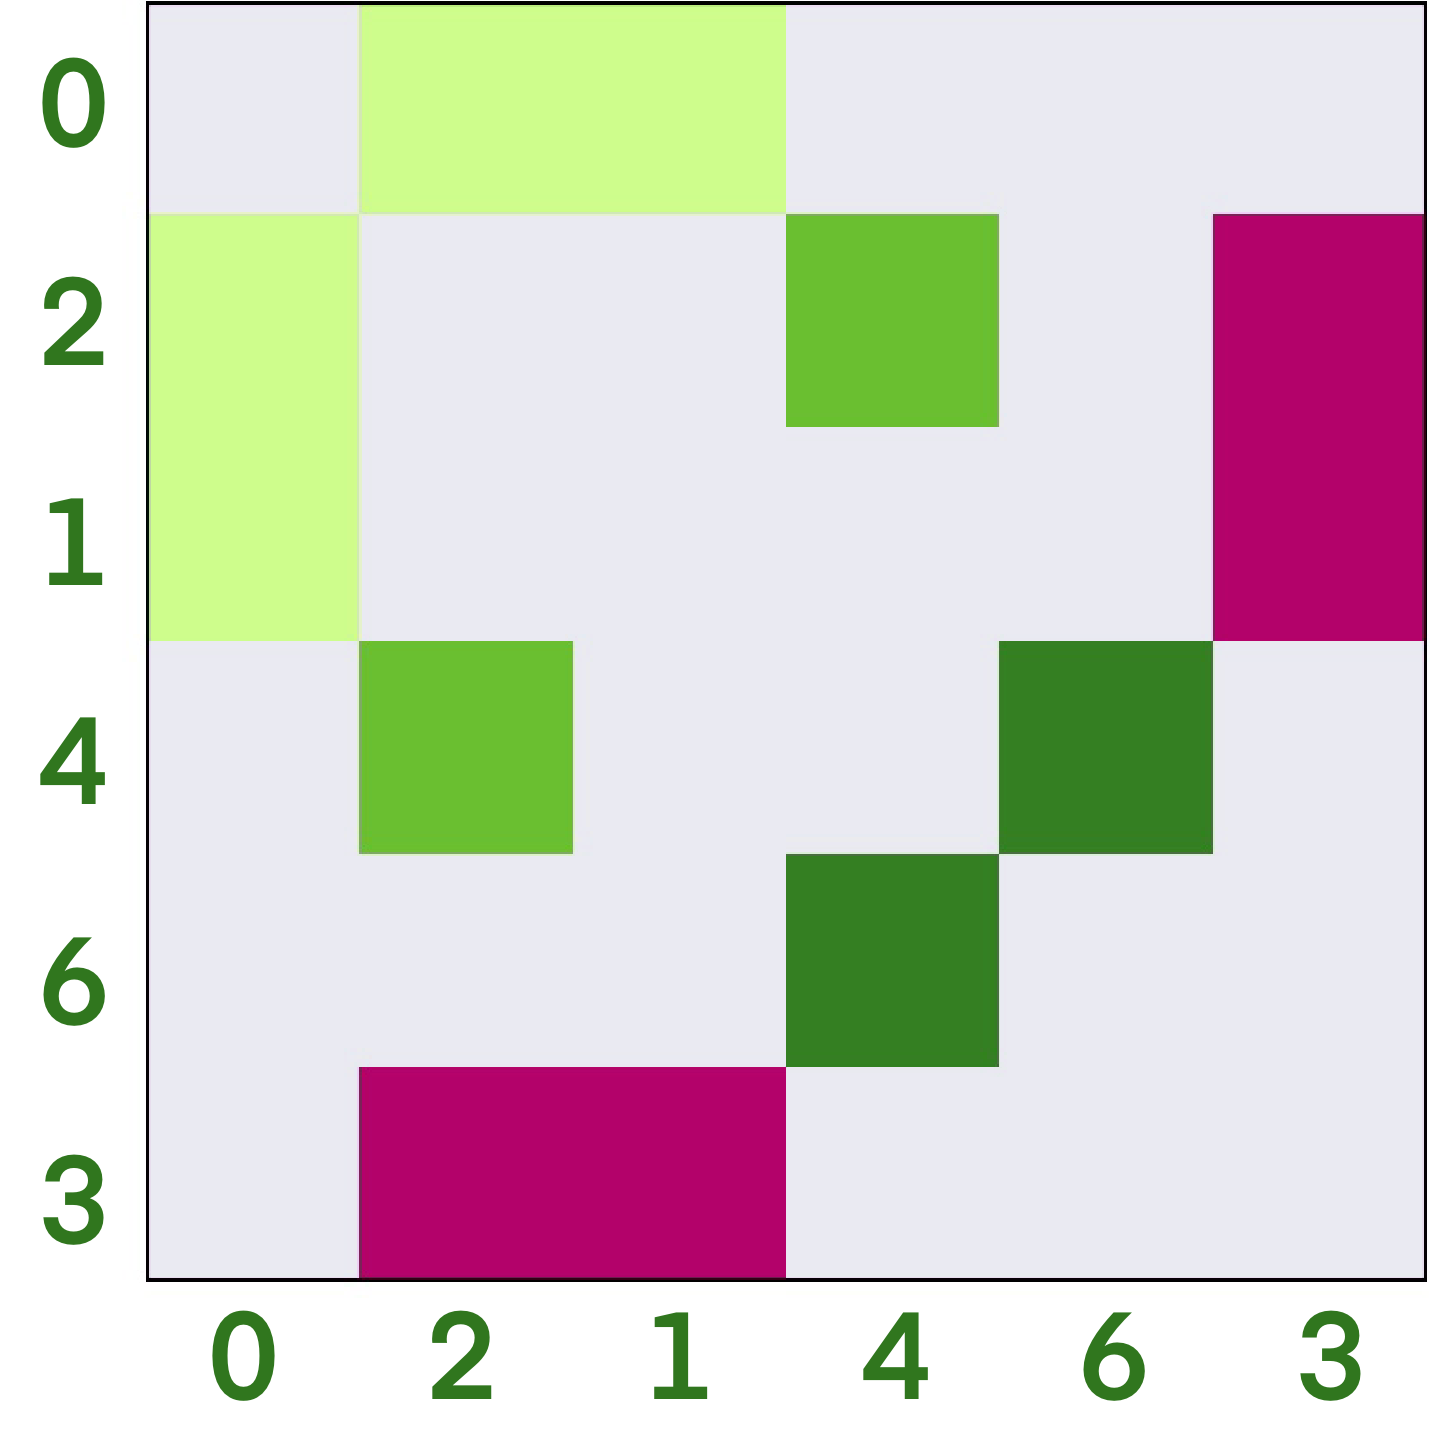
\includegraphics[width=\textwidth]{results/figures/dipole_yes_b.png}
        \caption{transition matrix for a 2D quantum dot when a magnetic field
            is applied.}
        \label{fig:transition_yes_b}
    \end{minipage}        
    \end{center}
\end{figure}

\begin{figure}
    \centering
    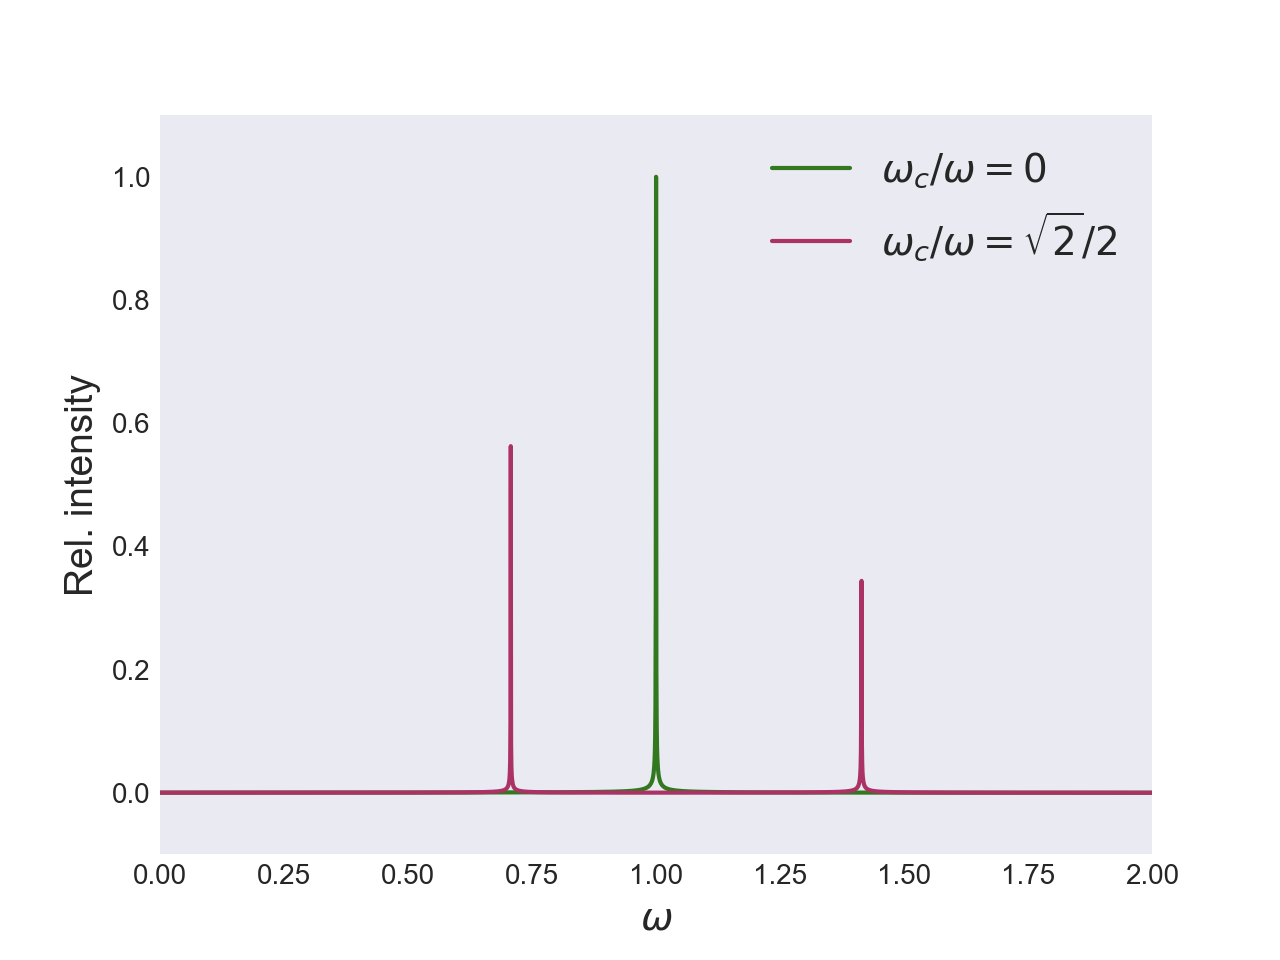
\includegraphics[width=0.75\textwidth]{results/figures/transmission_spectrum.png}
    \caption{Spectrum of a 2D quantum dot both with and without a magnetic field.}
    \label{fig:transmission_spectrum_b_field}
\end{figure}